\chapter{設計と実装}
本章では, 前章にて述べたMIWWGを実現する際の設計と実装について述べる。
また、本研究においては大きく分けて3つの技術を用いている。
市場における貨幣の役割を担うブロックチェーン技術、そのブロックチェーン技術の弱点であるトランザクション流通量の上限を引き上げるオフチェーン技術、IoTデータを実際に送信する役割のメッセージングシステム技術の3つである。
これら3つのうち各々をどのように用いたかについて、独立した節にて説明を行う。

\section{設計}
最初に、本節では設計について述べる。
\subsection{システム構成}
以下に、システム設計図\ref{SystemDesign}を示す。\\
\begin{figure}[htbp]
 \centering
  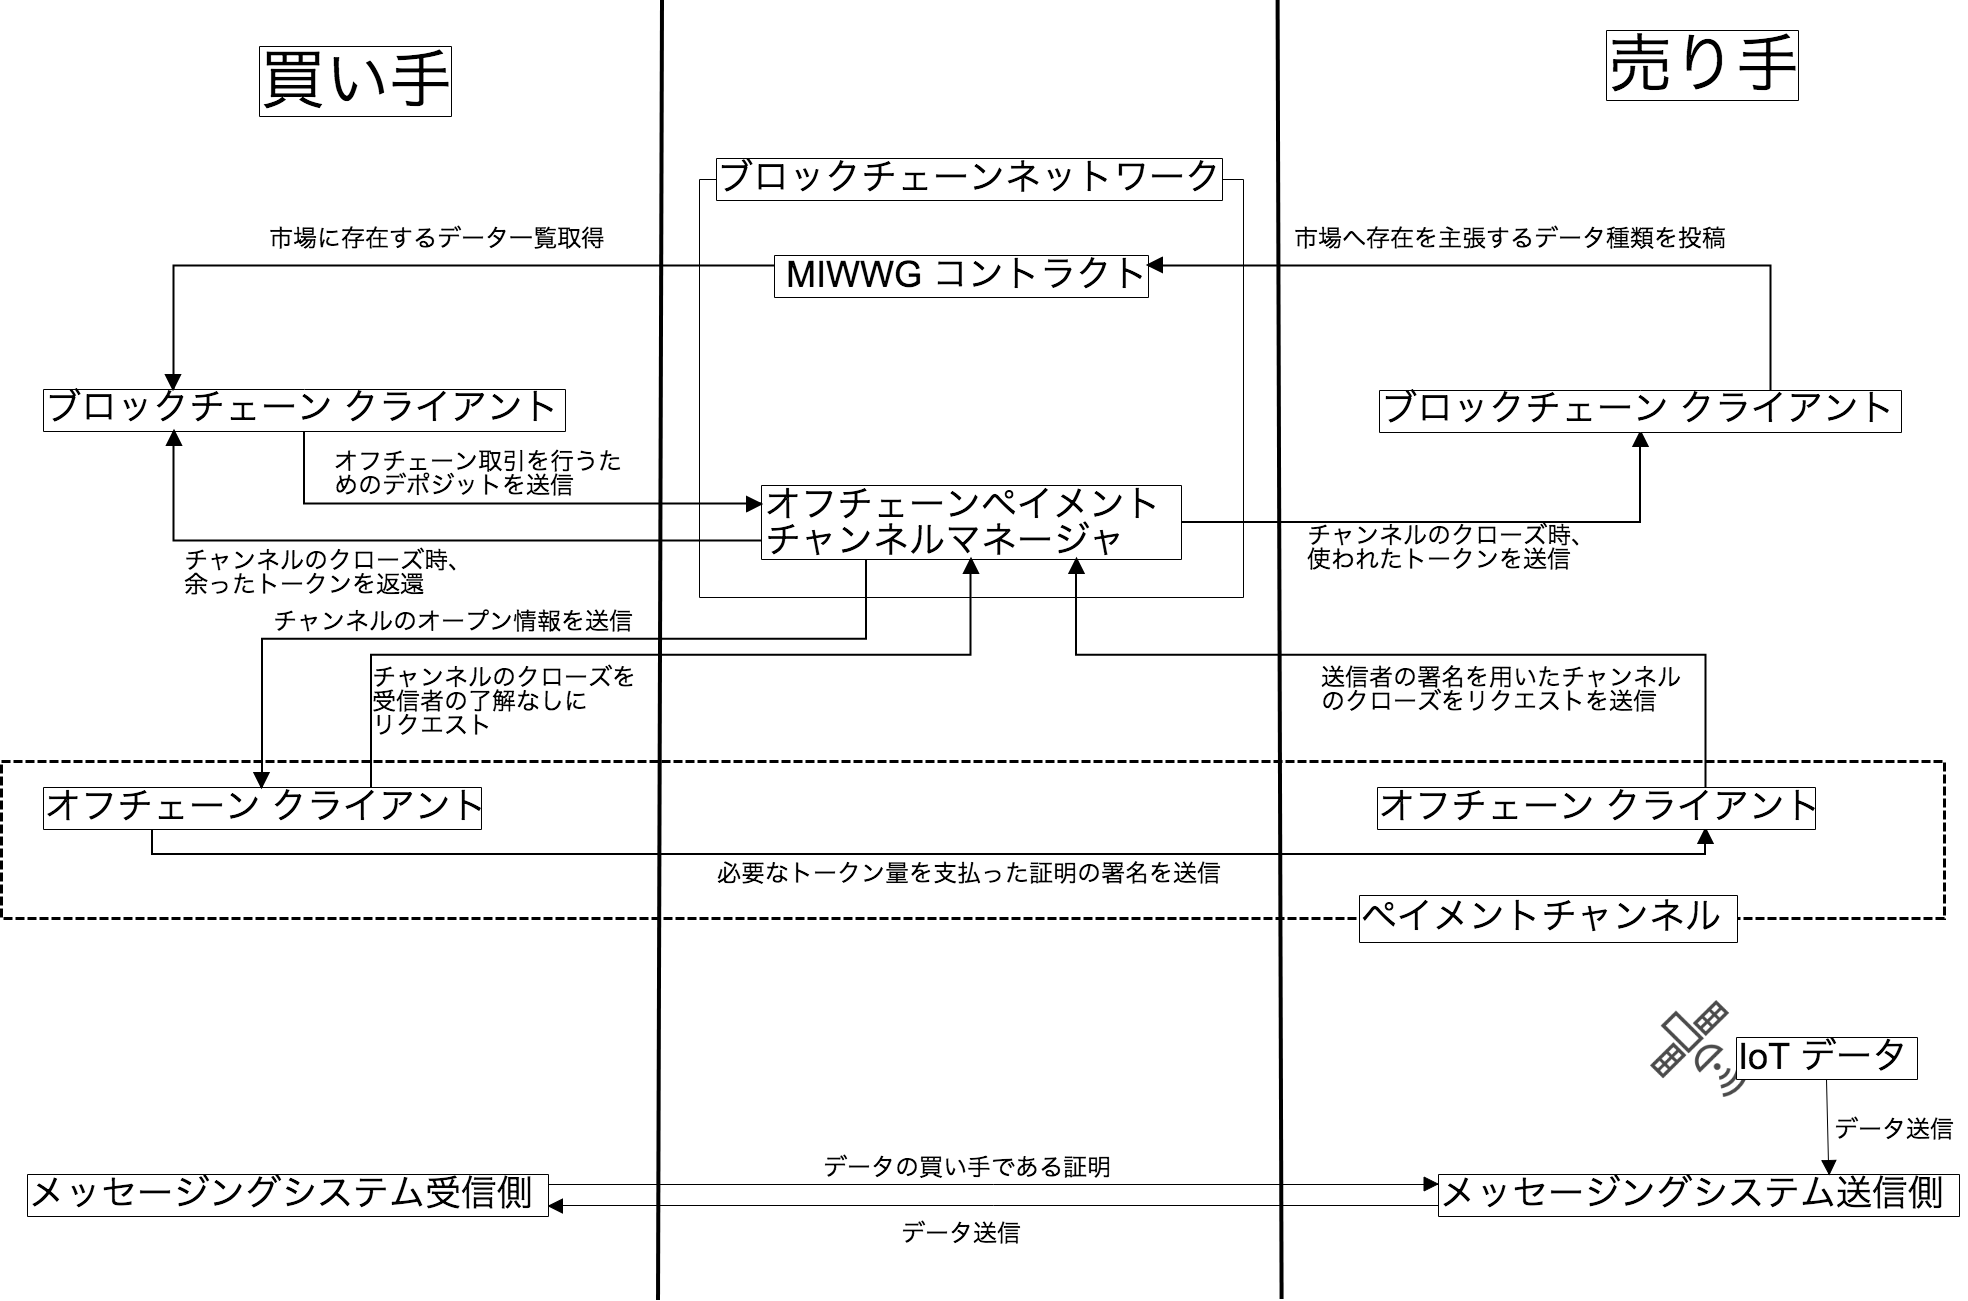
\includegraphics[width=160mm]{image/SystemDesign.png}
 \caption{システム設計図}
 \label{SystemDesign}
\end{figure}

\subsection{ブロックチェーン技術}
本研究において、ブロックチェーンのトークンが貨幣の役割を担い、ブロックチェーンはその元帳の役割を持つ。
一般に、ブロックチェーンはコントラクトを生成することが出来る。
そのコントラクト上にて、市場に存在するデータの管理やトークンの移動を行う。
データに関する情報のうち、多くの人にとって重要な定量的情報を列挙し、それをコントラクトの中に記述する。
本研究では以下の項目を定量的情報として入力させることとした。

\begin{itemize}
\item データの名前
\item 1つのデータあたりの値段
\item データが送られてくる間隔
\item トークン送信の遅延に関する許容時間
\item 前払いで必要なトークンの量
\item データの売り手のアドレス
\item データに関するその他の説明がある場合、それを記述するURL
\end{itemize}

1つのデータあたりの値段とデータが送られてくる間隔、データの売り手のアドレスはデータの買い手がトークンを利用する際に必要な情報である。
また、買い手が環境の悪いネットワーク環境下からデータを買おうとする場合、トークン送信の遅延に関する許容時間は重要なファクターとなる。
買い手に契約を終了する気持ちがなくとも、売り手がトークン送信の見送信を検知し、契約が終了となる可能性があるためである。
その場合、もう一度契約をオンチェーンの処理によって開始する必要があり、これは本来不必要であったマイナーへの手数料を必要とする。
前払いで必要なトークンの量は、契約を開始した後に直ぐに買い手がトークンを未送信にしてしまい、買い手がデータを遅延の許容時間分だけ無料で受信するのみで契約を終了してしまう行動を抑制するためのものである。
また、これらの定量的情報以外にデータに関する詳細な説明を記述する場合は、そのデータに関する情報を記載したURLをトランザクション内に記述する。
このことにより、このデータの存在を市場へ主張する際のトランザクションサイズを小さくする狙いがある。
一方、同じURLであってもそこに記載する内容はブロックに入った後も変更可能である。
従って、取引における重要な事項をこのURLに記述したとしても、それは信頼できるものではない。
あくまでURLの記述内容は他の項目にプラスして、データに関する内容を理解するために使われるものとなる。

\subsection{オフチェーン技術}
本研究において、オフチェーン技術はブロックチェーンの処理能力を補完するために使われる。
IoTデータは短い時間間隔で流れてくるデータであり、ブロックチェーンの処理能力では追いつかないためだ。
データ取引の開始時にオンチェーンにてデポジットを行い、ペイメントチャンネルをオープンし、その情報がオフチェーンクライアントへ渡る。
そしてデータの買い手は売り手へ新しいトークンバランスによる署名値を提出することで、データの売り手へトークンを渡す。
最後に、データの買い手か売り手のいずれかがチャンネルをクローズし、最終的にデポジットされたトークンを分配する。

\subsection{メッセージングシステム}
本研究において、メッセージングシステムはIoTデータの送信に使われる。
一般に、メッセージキューシステムに基づく分散メッセージングシステムは次のような特徴を持つ。
\begin{itemize}
\item 非同期のメッセージ送信が可能である。これにより送信側と受信側とのサービスが疎結合になり、片方の処理の遅延がもう一方に影響を与えるリスクが減る。
\item 送信を行う一つのノードが落ちたとしても、他のノードが直ぐに落ちたノードの代わりの役目を担う。これにより、可用性が高いことが担保される。
\item 送信側で新しくノードを追加した時、新規ノードを含めた協調動作が始まる。これにより、拡張性が高いことが担保され、より多くのメッセージ処理を裁くことが出来るような拡張を簡単にすることが出来る。
\end{itemize}
これらの特徴から、今回のIoTデータ市場の構築にはメッセージングシステムを使うことは最適である。
送信者と受信者のシステムが疎結合であり、各々の責任によってデータの送受信が可能なためだ。
また、メッセージングシステムによってはCAPの定理においてどの要素を重視するかをパラメタで指定することも可能であり、データの送受信者にとってよりフレキシブルな設定が可能となっている。\\
また、メッセージングシステムはkerberosや簡単なユーザID/パスワード認証などを用い、データの買い手のみへデータの提供をしなくてはならない。
そしてトークンの取引が停止されたことが検知された時からなるべく早く、データの送信を不許可にしなくてはならない。

\subsection{実装}
\subsection{システム構成}
以下に、システム構成図\ref{SystemImplement}を示す。\\
\begin{figure}[htbp]
 \centering
  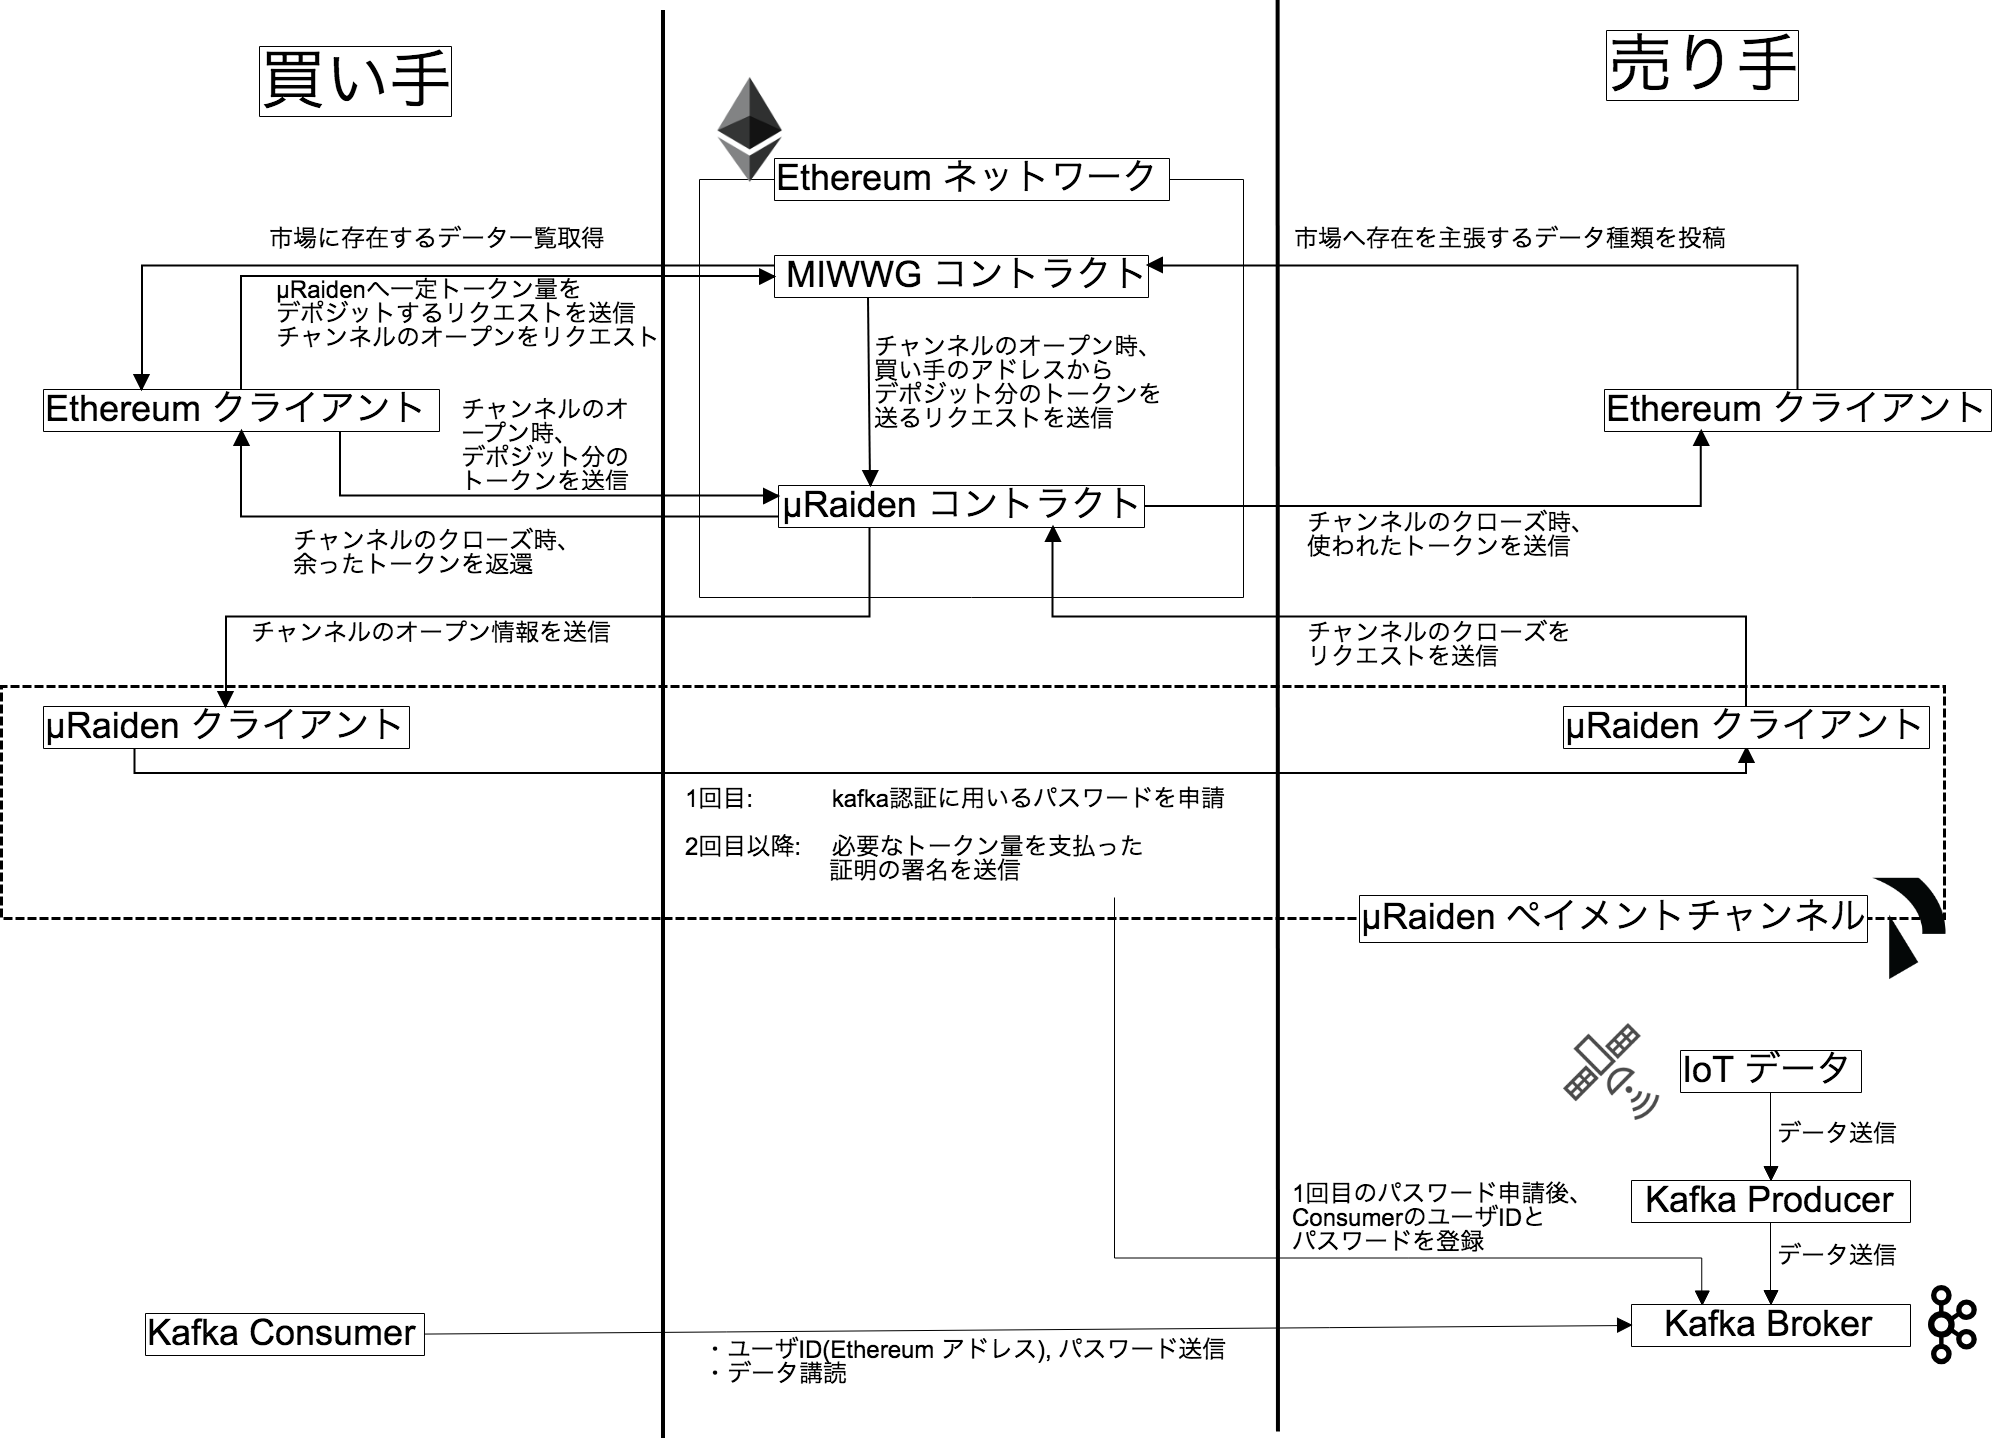
\includegraphics[width=160mm]{image/SystemImplement.png}
 \caption{システム構成図}
 \label{SystemImplement}
\end{figure}

\subsection{ブロックチェーン技術}
本研究では、ブロックチェーン技術の中からEthereumを利用する。
また、そのEthereumクライアントとして、go言語による実装であるgo-ethereum(以下、geth)を利用した。
ここでgethのオリジナルコードとは、gethのgithubレポジトリ(https://github.com/ethereum/go-ethereum)のConstant (v1.8.20)のことである。
solidityは0.4.17のバージョンを利用している。
最初に開発したトークンの中身について記述する。
採用したトークン規格はERC20に次ぐトークンの規格であるERC223を考慮しつつ、一部を改変して利用した。
これはERC223が本研究で採用するオフチェーン技術であるμRaidenがより薦める方式であるためである。
既存のERC20と比べて、コントラクトアドレスに対して誤ってトークンを送った時に取り戻せるtokenFallback関数が追加され、コントラクトに対するトランザクションとユーザに対するトランザクションを同じように捌けるようになっている。
これによりEthereumの掲げる理想である相手がコードか人間か気にせずにトークンのやり取りが出来るという世界をより体現しているものである。
このERC223の一般的な実装物はgithubのレポジトリであるDexaran/ERC223-token-standard(https://github.com/Dexaran/ERC223-token-standard)に存在する。
この元のソースコードに加える形で本研究では以下の構造体によってIoTデータを格納可能とした。
\begin{lstlisting}[caption=solidityによるデータを保持する構造体,label=DataNode]
struct DataNode {
  string name;  // データの名前
  uint256 price;  // 1つのデータあたりの値段
  uint256 interval;  // データが送られてくる間隔
  uint256 delay_permission_time;  // トークン送信の遅延に関する許容時間
  uint256 prepaid_value;  // 前払いで必要なトークンの量
  address author;  // データの売り手のアドレス
  string explanation_url;  // データに関するその他の説明がある場合、それを記述するURL
  uint256 data_index;  // 本データがデータ市場において一意に定まるID。1から順番にインクリメントされていく。
}
\end{lstlisting}
以上がIoTデータの種類を格納する構造である。
また、この他にEthereumトークンを本トークンへ変換することのできる機能を実装した。本トークンはEthereumの1wei = 1MI(本トークンの通貨単位)としてEthereumネットワーク上で動くものである。
さらに、一般的なtransfer(\_to, \_value, \_data)の関数をラップするbuyData関数を作ることによって、μRaidenクライアントから何のデータを買いたいかについて、買い手からの情報を得る実装を行なっている。以下がその様子である。
\begin{lstlisting}[caption=gethのEIP155のフォーク確認機能の削除 params/config.go ,label=DataNode]
uint256[] user_bought_log; // ユーザの購入履歴を格納
function buyData(
    address _to,
    uint256 _value,
    bytes _data,
    uint256 data_index)
    public
    returns (bool)
{
    user_bought_log.push(data_index); // ユーザの購入履歴に追加
    emit boughtData(msg.sender, data_index);  // ユーザの購入が行われたことを示すeventを送出
    bool ret = transfer(_to, _value, _data);  // ERC223対応のtransfer関数を実行
    return ret
    }
\end{lstlisting}
これにより、一つのトランザクションによってデータの購買とそれに関するペイメントチャンネルを開くという二つの行為ができるようになっている。 \\
次に今回使用したgethに加えた変更について述べる。
今回はプライベートネットワークで動作を検証するにあたり、gethがμRaidenの発行するEIP155を考慮した署名のトランザクションを捌かないという事象が発生した。
これはリプレイアタックを防ぐためのものであり、Ethereumのブロックナンバーが2675000以降のものについてのみEIP155を適用する実装がなされていた。
しかし、これではトランザクションが裁かれ始めるまでに大量の時間を要してしまうため、この機能を簡単に削除した。
\begin{lstlisting}[caption=gethのEIP155のフォーク確認機能の削除 params/config.go ,label=EIP155]
227 // IsEIP155 returns whether num is either equal to the EIP155 fork block or greater.
228 func (c *ChainConfig) IsEIP155(num *big.Int) bool {
229     //return isForked(c.EIP155Block, num) // 既存の判別箇所を削除
230     return true // 全てのEIP155署名のトランザクションが裁かれるように変更
231 }
\end{lstlisting}

\subsection{オフチェーン技術}
オフチェーン技術について、本研究ではμRaiden(https://github.com/raiden-network/microraiden)の0.2.0を使用した。
このμRaidenについて、いくつかの変更を加えている。
最初に、ペイメントチャンネルをオープンするためにMIWWGコントラクトへtransfer関数を実行する際、独自の関数であるbuyData関数を呼び出している。
\begin{lstlisting}[caption=μRaidenクライアントの変更 client/client.py  ,label=RaidenOpenChannel]
def open_channel(self, receiver_address: str, deposit: int):
    data = decode_hex(self.context.address) + decode_hex(receiver_address)
    tx = create_signed_contract_transaction(
        self.context.private_key,
        self.context.token,
        # 'transfer', //オリジナル部分
        'buyData', // 追加部分
        [
            self.context.channel_manager.address,
            deposit,
            data,
            data_index // 追加部分
        ]
    )
\end{lstlisting}
上記と同じ変更をペイメントチャンネルへのデポジットを増やす際に使用するtopup関数にも加えている。
また、デフォルトの設定で用いるとethereumのテストネットワークへと繋がってしまい、プライベートネットワークに繋がらない。
よって以下の変更を加えた。
\begin{lstlisting}[caption=ネットワーク設定の変更 config.py  ,label=RaidenOpenChannel]
 40 # network-specific configuration
 41 NETWORK_CONFIG_DEFAULTS = {
 ...
 63     # private MIWWG //63行目から67行目まで追加部分
 64     98: NetworkConfig(
 65         channel_manager_address='0xd0c19d7d41ae4a5561d2289d997da00b9de1bf73',
 66         start_sync_block=0
 67     ),
 ...
104    #NETWORK_CFG.set_defaults(3)  // デフォルトのネットワークID
104    NETWORK_CFG.set_defaults(98)  // 今回使用するネットワークID
\end{lstlisting}
また、μRaidenはバックエンドのDBとしてsqliteを使用している。
このDBを使って、のちにメッセージングシステムにてユーザIDとパスワードを使用した認証を行う。
そのパスワードを保持する目的と、μRaidenでは想定されていない同じ送り手と受取り手のアドレスに対して複数の別のペイメントを使用することから、DB構造について変更を加えている。
\begin{lstlisting}[caption=DB構造の変更 channel\_manager/state.py  ,label=sqliteSql]
CREATE TABLE `channels` (
    `sender`            CHAR(42)        NOT NULL,
    `data\_index`            INTEGER        NOT NULL,  # 追加
    `password`            CHAR(42)        NOT NULL,  # 追加
    `open_block_number` INTEGER         NOT NULL,
    `deposit`           DECIMAL(78,0)   NOT NULL,
    `balance`           DECIMAL(78,0)   NOT NULL,
    `last_signature`    CHAR(132),
    `settle_timeout`    INTEGER         NOT NULL,
    `mtime`             INTEGER         NOT NULL,
    `ctime`             INTEGER         NOT NULL,
    `state`             INTEGER         NOT NULL,
    `confirmed`         BOOL            NOT NULL,
    PRIMARY KEY (`sender`, `open_block_number`, `data_index`)  # 最後の要素について、追加
);
\end{lstlisting}
またこれに伴い、このDBを利用するコードについても全て変更を加えている。
他の機能として、パスワードを登録する際にアクセスするapiのエンドポイントを作成している。
WebサーバはgeventのpywsgiにあるWSGIServerを用い、その上でflaskを使い、ルーティングを行なっている。

\subsection{メッセージングシステム}
本実装では、JVM上にて動作するkafkaをメッセージングシステムとして用いている。
kafkaはconsumerとbroker, producerからなり、各々がデータの受け手、コーディネイター、送り手である。
各々でクラスターが構成可能で、可用性に優れたメッセージングシステムであるため、本研究にて用いた、
バージョンであるが、このkafka内におけるSASL\_PLAIN認証を用いてユーザ認証を行うものの、現状の最新バージョンである2.1.0や2.0.0ではこの認証が動作しなかった。
したがってメジャーダウングレードを行い、1.0.2のバージョンを用いている。
また、scalaは2.12のバージョンを用いている。
そしてユーザ認証は以下のconfファイルを用いたSASL認証を使用している。
\begin{lstlisting}[caption=SASL認証の設定 config/producer.properties  ,label=serverProperties]
sasl.mechanism=PLAIN
security.protocol=SASL_PLAINTEXT
sasl.jaas.config=org.apache.kafka.common.security.plain.PlainLoginModule required \
  username="yoshiyuki" \
  password="yoshiyuki-secret";
\end{lstlisting}
また、JVMを立ち上げた後でも、このファイルにユーザ記述部分を足すことでkafkaへ動的にユーザの追加が出来る。
これにより、新しいユーザの追加を行っている。
また、シェルを経由してbin/kafka-acls.shを用いることで動的にユーザの権限の制限が可能となる。
これにより、トークンを送信してこなくなったユーザからデータを購読する権限を剥奪している。 \\
また、kafkaはCAPの定理におけるCAを満たすものであり、PであるPartition Tolerance(分断耐性)は低いものである。
これについて、kafkaは本来は同一データセンター内にて用いられることが前提のプロダクトであり、分断される可能性が低いので問題ないとしている。
しかし、今回のユースケースではkafkaのproducerとconsumerは同一データセンター内に存在しないことの方が多い。
つまり、ネットワークが分断される可能性は十分に考えられるのだ。
そこでacksというパラメタが設定できる。
ここではレプリケーションされたメッセージがいくつ送信成功することを要求するかを指定でき、これにallを指定すると全てのレプリケーションを格納するbrokerに情報が書き込まれることを、producerが要求することとなる。
さらにreplication.factorによってそのメッセージをいくつのbrokerが持つかについて指定することができる。
これらをallや大きな数字に設定を行うと、あるbrokerとconsumerの分断が起こったとしても他のネットワークを用いてデータの配信は可能なままである。
このように、kafkaではAのAvailability(可用性)を犠牲にすることでPの分断耐性を増すことが可能であり、今回のユースケースではPを増すことを考慮する必要がある。

\section{まとめ}
本章では本研究にて用いるブロックチェーン技術や、それをIoTデータのような短い間隔の支払いが必要な場合に対応するためのオフチェーン技術、そしてデータを多くのスループットで拡張性を保持しつつ送受信するメッセージングシステムについて述べた。